\documentclass[11pt]{book}              % Book class in 11 points
%\documentclass[justified,twoside]{tufte-book}


\parindent0pt  \parskip10pt             % make block paragraphs
%\raggedright                            % do not right justify
\usepackage{xcolor}
\usepackage{amsmath}
\usepackage{amssymb}
\usepackage[round]{natbib}
\usepackage{graphicx}
\usepackage{amsthm}
\usepackage{tgpagella}
\usepackage{emptypage}
\usepackage{multirow}
\usepackage{booktabs}
\usepackage[LGR,T1]{fontenc}
\newcommand{\textgreek}[1]{\begingroup\fontencoding{LGR}\selectfont#1\endgroup}

\usepackage{tcolorbox}


\usepackage{microtype}


\definecolor{echodrk}{HTML}{0099cc}
\definecolor{mymauve}{rgb}{0.58,0,0.82}
\usepackage[colorlinks,linkcolor=mymauve,citecolor=echodrk]{hyperref}

\definecolor{boxgray}{rgb}{0.9,0.9,0.9}
\definecolor{boxpink}{rgb}{0.9,0.7,0.7}

\renewcommand\vec{\mathbf}
\newcommand\mat{\mathbf}

\makeatletter
\renewcommand{\thesection}{%
  \ifnum\c@chapter<1 \@arabic\c@section
  \else \thechapter.\@arabic\c@section
  \fi
}
\makeatother



% margin notes
%\usepackage[top=1.5cm, bottom=1.5cm, outer=5cm, inner=2cm, heightrounded, marginparwidth=2.5cm, marginparsep=2cm]{geometry}
\usepackage{marginnote}
\renewcommand*{\marginfont}{\footnotesize} %\justify} <- Taco: including \justify will throw errors.

 \newcommand{\joan}[1]{{\color{green}#1}}
 \newcommand{\michael}[1]{{\color{magenta}#1}} \newcommand{\taco}[1]{{\color{blue}#1}}
 \newcommand{\petar}[1]{{\color{cyan}#1}}
%\newcommand{\joan}[1]{{#1}}
%\newcommand{\michael}[1]{{#1}}
%\newcommand{\taco}[1]{{#1}}
%\newcommand{\petar}[1]{{#1}}


%%%%% NEW MATH DEFINITIONS %%%%%

\usepackage{amsmath,amsfonts,bm}

% Mark sections of captions for referring to divisions of figures
\newcommand{\figleft}{{\em (Left)}}
\newcommand{\figcenter}{{\em (Center)}}
\newcommand{\figright}{{\em (Right)}}
\newcommand{\figtop}{{\em (Top)}}
\newcommand{\figbottom}{{\em (Bottom)}}
\newcommand{\captiona}{{\em (a)}}
\newcommand{\captionb}{{\em (b)}}
\newcommand{\captionc}{{\em (c)}}
\newcommand{\captiond}{{\em (d)}}

% Highlight a newly defined term
\newcommand{\newterm}[1]{{\bf #1}}


% Figure reference, lower-case.
\def\figref#1{figure~\ref{#1}}
% Figure reference, capital. For start of sentence
\def\Figref#1{Figure~\ref{#1}}
\def\twofigref#1#2{figures \ref{#1} and \ref{#2}}
\def\quadfigref#1#2#3#4{figures \ref{#1}, \ref{#2}, \ref{#3} and \ref{#4}}
% Section reference, lower-case.
\def\secref#1{section~\ref{#1}}
% Section reference, capital.
\def\Secref#1{Section~\ref{#1}}
% Reference to two sections.
\def\twosecrefs#1#2{sections \ref{#1} and \ref{#2}}
% Reference to three sections.
\def\secrefs#1#2#3{sections \ref{#1}, \ref{#2} and \ref{#3}}
% Reference to an equation, lower-case.
% \def\eqref#1{equation~\ref{#1}}
\def\eqref#1{(\ref{#1})}
% Reference to an equation, upper case
\def\Eqref#1{Equation~\ref{#1}}
% A raw reference to an equation---avoid using if possible
\def\plaineqref#1{\ref{#1}}
% Reference to a chapter, lower-case.
\def\chapref#1{chapter~\ref{#1}}
% Reference to an equation, upper case.
\def\Chapref#1{Chapter~\ref{#1}}
% Reference to a range of chapters
\def\rangechapref#1#2{chapters\ref{#1}--\ref{#2}}
% Reference to an algorithm, lower-case.
\def\algref#1{algorithm~\ref{#1}}
% Reference to an algorithm, upper case.
\def\Algref#1{Algorithm~\ref{#1}}
\def\twoalgref#1#2{algorithms \ref{#1} and \ref{#2}}
\def\Twoalgref#1#2{Algorithms \ref{#1} and \ref{#2}}
% Reference to a part, lower case
\def\partref#1{part~\ref{#1}}
% Reference to a part, upper case
\def\Partref#1{Part~\ref{#1}}
\def\twopartref#1#2{parts \ref{#1} and \ref{#2}}

\def\ceil#1{\lceil #1 \rceil}
\def\floor#1{\lfloor #1 \rfloor}
\def\1{\bm{1}}
\newcommand{\train}{\mathcal{D}}
\newcommand{\valid}{\mathcal{D_{\mathrm{valid}}}}
\newcommand{\test}{\mathcal{D_{\mathrm{test}}}}

\def\eps{{\epsilon}}


% Random variables
\def\reta{{\textnormal{$\eta$}}}
\def\ra{{\textnormal{a}}}
\def\rb{{\textnormal{b}}}
\def\rc{{\textnormal{c}}}
\def\rd{{\textnormal{d}}}
\def\re{{\textnormal{e}}}
\def\rf{{\textnormal{f}}}
\def\rg{{\textnormal{g}}}
\def\rh{{\textnormal{h}}}
\def\ri{{\textnormal{i}}}
\def\rj{{\textnormal{j}}}
\def\rk{{\textnormal{k}}}
\def\rl{{\textnormal{l}}}
% rm is already a command, just don't name any random variables m
\def\rn{{\textnormal{n}}}
\def\ro{{\textnormal{o}}}
\def\rp{{\textnormal{p}}}
\def\rq{{\textnormal{q}}}
\def\rr{{\textnormal{r}}}
\def\rs{{\textnormal{s}}}
\def\rt{{\textnormal{t}}}
\def\ru{{\textnormal{u}}}
\def\rv{{\textnormal{v}}}
\def\rw{{\textnormal{w}}}
\def\rx{{\textnormal{x}}}
\def\ry{{\textnormal{y}}}
\def\rz{{\textnormal{z}}}

% Random vectors
\def\rvepsilon{{\mathbf{\epsilon}}}
\def\rvtheta{{\mathbf{\theta}}}
\def\rva{{\mathbf{a}}}
\def\rvb{{\mathbf{b}}}
\def\rvc{{\mathbf{c}}}
\def\rvd{{\mathbf{d}}}
\def\rve{{\mathbf{e}}}
\def\rvf{{\mathbf{f}}}
\def\rvg{{\mathbf{g}}}
\def\rvh{{\mathbf{h}}}
\def\rvu{{\mathbf{i}}}
\def\rvj{{\mathbf{j}}}
\def\rvk{{\mathbf{k}}}
\def\rvl{{\mathbf{l}}}
\def\rvm{{\mathbf{m}}}
\def\rvn{{\mathbf{n}}}
\def\rvo{{\mathbf{o}}}
\def\rvp{{\mathbf{p}}}
\def\rvq{{\mathbf{q}}}
\def\rvr{{\mathbf{r}}}
\def\rvs{{\mathbf{s}}}
\def\rvt{{\mathbf{t}}}
\def\rvu{{\mathbf{u}}}
\def\rvv{{\mathbf{v}}}
\def\rvw{{\mathbf{w}}}
\def\rvx{{\mathbf{x}}}
\def\rvy{{\mathbf{y}}}
\def\rvz{{\mathbf{z}}}

% Elements of random vectors
\def\erva{{\textnormal{a}}}
\def\ervb{{\textnormal{b}}}
\def\ervc{{\textnormal{c}}}
\def\ervd{{\textnormal{d}}}
\def\erve{{\textnormal{e}}}
\def\ervf{{\textnormal{f}}}
\def\ervg{{\textnormal{g}}}
\def\ervh{{\textnormal{h}}}
\def\ervi{{\textnormal{i}}}
\def\ervj{{\textnormal{j}}}
\def\ervk{{\textnormal{k}}}
\def\ervl{{\textnormal{l}}}
\def\ervm{{\textnormal{m}}}
\def\ervn{{\textnormal{n}}}
\def\ervo{{\textnormal{o}}}
\def\ervp{{\textnormal{p}}}
\def\ervq{{\textnormal{q}}}
\def\ervr{{\textnormal{r}}}
\def\ervs{{\textnormal{s}}}
\def\ervt{{\textnormal{t}}}
\def\ervu{{\textnormal{u}}}
\def\ervv{{\textnormal{v}}}
\def\ervw{{\textnormal{w}}}
\def\ervx{{\textnormal{x}}}
\def\ervy{{\textnormal{y}}}
\def\ervz{{\textnormal{z}}}

% Random matrices
\def\rmA{{\mathbf{A}}}
\def\rmB{{\mathbf{B}}}
\def\rmC{{\mathbf{C}}}
\def\rmD{{\mathbf{D}}}
\def\rmE{{\mathbf{E}}}
\def\rmF{{\mathbf{F}}}
\def\rmG{{\mathbf{G}}}
\def\rmH{{\mathbf{H}}}
\def\rmI{{\mathbf{I}}}
\def\rmJ{{\mathbf{J}}}
\def\rmK{{\mathbf{K}}}
\def\rmL{{\mathbf{L}}}
\def\rmM{{\mathbf{M}}}
\def\rmN{{\mathbf{N}}}
\def\rmO{{\mathbf{O}}}
\def\rmP{{\mathbf{P}}}
\def\rmQ{{\mathbf{Q}}}
\def\rmR{{\mathbf{R}}}
\def\rmS{{\mathbf{S}}}
\def\rmT{{\mathbf{T}}}
\def\rmU{{\mathbf{U}}}
\def\rmV{{\mathbf{V}}}
\def\rmW{{\mathbf{W}}}
\def\rmX{{\mathbf{X}}}
\def\rmY{{\mathbf{Y}}}
\def\rmZ{{\mathbf{Z}}}

% Elements of random matrices
\def\ermA{{\textnormal{A}}}
\def\ermB{{\textnormal{B}}}
\def\ermC{{\textnormal{C}}}
\def\ermD{{\textnormal{D}}}
\def\ermE{{\textnormal{E}}}
\def\ermF{{\textnormal{F}}}
\def\ermG{{\textnormal{G}}}
\def\ermH{{\textnormal{H}}}
\def\ermI{{\textnormal{I}}}
\def\ermJ{{\textnormal{J}}}
\def\ermK{{\textnormal{K}}}
\def\ermL{{\textnormal{L}}}
\def\ermM{{\textnormal{M}}}
\def\ermN{{\textnormal{N}}}
\def\ermO{{\textnormal{O}}}
\def\ermP{{\textnormal{P}}}
\def\ermQ{{\textnormal{Q}}}
\def\ermR{{\textnormal{R}}}
\def\ermS{{\textnormal{S}}}
\def\ermT{{\textnormal{T}}}
\def\ermU{{\textnormal{U}}}
\def\ermV{{\textnormal{V}}}
\def\ermW{{\textnormal{W}}}
\def\ermX{{\textnormal{X}}}
\def\ermY{{\textnormal{Y}}}
\def\ermZ{{\textnormal{Z}}}

% Vectors
\def\vzero{{\bm{0}}}
\def\vone{{\bm{1}}}
\def\vmu{{\bm{\mu}}}
\def\vtheta{{\bm{\theta}}}
\def\va{{\bm{a}}}
\def\vb{{\bm{b}}}
\def\vc{{\bm{c}}}
\def\vd{{\bm{d}}}
\def\ve{{\bm{e}}}
\def\vf{{\bm{f}}}
\def\vg{{\bm{g}}}
\def\vh{{\bm{h}}}
\def\vi{{\bm{i}}}
\def\vj{{\bm{j}}}
\def\vk{{\bm{k}}}
\def\vl{{\bm{l}}}
\def\vm{{\bm{m}}}
\def\vn{{\bm{n}}}
\def\vo{{\bm{o}}}
\def\vp{{\bm{p}}}
\def\vq{{\bm{q}}}
\def\vr{{\bm{r}}}
\def\vs{{\bm{s}}}
\def\vt{{\bm{t}}}
\def\vu{{\bm{u}}}
\def\vv{{\bm{v}}}
\def\vw{{\bm{w}}}
\def\vx{{\bm{x}}}
\def\vy{{\bm{y}}}
\def\vz{{\bm{z}}}

% Elements of vectors
\def\evalpha{{\alpha}}
\def\evbeta{{\beta}}
\def\evepsilon{{\epsilon}}
\def\evlambda{{\lambda}}
\def\evomega{{\omega}}
\def\evmu{{\mu}}
\def\evpsi{{\psi}}
\def\evsigma{{\sigma}}
\def\evtheta{{\theta}}
\def\eva{{a}}
\def\evb{{b}}
\def\evc{{c}}
\def\evd{{d}}
\def\eve{{e}}
\def\evf{{f}}
\def\evg{{g}}
\def\evh{{h}}
\def\evi{{i}}
\def\evj{{j}}
\def\evk{{k}}
\def\evl{{l}}
\def\evm{{m}}
\def\evn{{n}}
\def\evo{{o}}
\def\evp{{p}}
\def\evq{{q}}
\def\evr{{r}}
\def\evs{{s}}
\def\evt{{t}}
\def\evu{{u}}
\def\evv{{v}}
\def\evw{{w}}
\def\evx{{x}}
\def\evy{{y}}
\def\evz{{z}}

% Matrix
\def\mA{{\bm{A}}}
\def\mB{{\bm{B}}}
\def\mC{{\bm{C}}}
\def\mD{{\bm{D}}}
\def\mE{{\bm{E}}}
\def\mF{{\bm{F}}}
\def\mG{{\bm{G}}}
\def\mH{{\bm{H}}}
\def\mI{{\bm{I}}}
\def\mJ{{\bm{J}}}
\def\mK{{\bm{K}}}
\def\mL{{\bm{L}}}
\def\mM{{\bm{M}}}
\def\mN{{\bm{N}}}
\def\mO{{\bm{O}}}
\def\mP{{\bm{P}}}
\def\mQ{{\bm{Q}}}
\def\mR{{\bm{R}}}
\def\mS{{\bm{S}}}
\def\mT{{\bm{T}}}
\def\mU{{\bm{U}}}
\def\mV{{\bm{V}}}
\def\mW{{\bm{W}}}
\def\mX{{\bm{X}}}
\def\mY{{\bm{Y}}}
\def\mZ{{\bm{Z}}}
\def\mBeta{{\bm{\beta}}}
\def\mPhi{{\bm{\Phi}}}
\def\mLambda{{\bm{\Lambda}}}
\def\mSigma{{\bm{\Sigma}}}

% Tensor
\DeclareMathAlphabet{\mathsfit}{\encodingdefault}{\sfdefault}{m}{sl}
\SetMathAlphabet{\mathsfit}{bold}{\encodingdefault}{\sfdefault}{bx}{n}
\newcommand{\tens}[1]{\bm{\mathsfit{#1}}}
\def\tA{{\tens{A}}}
\def\tB{{\tens{B}}}
\def\tC{{\tens{C}}}
\def\tD{{\tens{D}}}
\def\tE{{\tens{E}}}
\def\tF{{\tens{F}}}
\def\tG{{\tens{G}}}
\def\tH{{\tens{H}}}
\def\tI{{\tens{I}}}
\def\tJ{{\tens{J}}}
\def\tK{{\tens{K}}}
\def\tL{{\tens{L}}}
\def\tM{{\tens{M}}}
\def\tN{{\tens{N}}}
\def\tO{{\tens{O}}}
\def\tP{{\tens{P}}}
\def\tQ{{\tens{Q}}}
\def\tR{{\tens{R}}}
\def\tS{{\tens{S}}}
\def\tT{{\tens{T}}}
\def\tU{{\tens{U}}}
\def\tV{{\tens{V}}}
\def\tW{{\tens{W}}}
\def\tX{{\tens{X}}}
\def\tY{{\tens{Y}}}
\def\tZ{{\tens{Z}}}


% Graph
\def\gA{{\mathcal{A}}}
\def\gB{{\mathcal{B}}}
\def\gC{{\mathcal{C}}}
\def\gD{{\mathcal{D}}}
\def\gE{{\mathcal{E}}}
\def\gF{{\mathcal{F}}}
\def\gG{{\mathcal{G}}}
\def\gH{{\mathcal{H}}}
\def\gI{{\mathcal{I}}}
\def\gJ{{\mathcal{J}}}
\def\gK{{\mathcal{K}}}
\def\gL{{\mathcal{L}}}
\def\gM{{\mathcal{M}}}
\def\gN{{\mathcal{N}}}
\def\gO{{\mathcal{O}}}
\def\gP{{\mathcal{P}}}
\def\gQ{{\mathcal{Q}}}
\def\gR{{\mathcal{R}}}
\def\gS{{\mathcal{S}}}
\def\gT{{\mathcal{T}}}
\def\gU{{\mathcal{U}}}
\def\gV{{\mathcal{V}}}
\def\gW{{\mathcal{W}}}
\def\gX{{\mathcal{X}}}
\def\gY{{\mathcal{Y}}}
\def\gZ{{\mathcal{Z}}}

% Sets
\def\sA{{\mathbb{A}}}
\def\sB{{\mathbb{B}}}
\def\sC{{\mathbb{C}}}
\def\sD{{\mathbb{D}}}
% Don't use a set called E, because this would be the same as our symbol
% for expectation.
\def\sF{{\mathbb{F}}}
\def\sG{{\mathbb{G}}}
\def\sH{{\mathbb{H}}}
\def\sI{{\mathbb{I}}}
\def\sJ{{\mathbb{J}}}
\def\sK{{\mathbb{K}}}
\def\sL{{\mathbb{L}}}
\def\sM{{\mathbb{M}}}
\def\sN{{\mathbb{N}}}
\def\sO{{\mathbb{O}}}
\def\sP{{\mathbb{P}}}
\def\sQ{{\mathbb{Q}}}
\def\sR{{\mathbb{R}}}
\def\sS{{\mathbb{S}}}
\def\sT{{\mathbb{T}}}
\def\sU{{\mathbb{U}}}
\def\sV{{\mathbb{V}}}
\def\sW{{\mathbb{W}}}
\def\sX{{\mathbb{X}}}
\def\sY{{\mathbb{Y}}}
\def\sZ{{\mathbb{Z}}}

% Entries of a matrix
\def\emLambda{{\Lambda}}
\def\emA{{A}}
\def\emB{{B}}
\def\emC{{C}}
\def\emD{{D}}
\def\emE{{E}}
\def\emF{{F}}
\def\emG{{G}}
\def\emH{{H}}
\def\emI{{I}}
\def\emJ{{J}}
\def\emK{{K}}
\def\emL{{L}}
\def\emM{{M}}
\def\emN{{N}}
\def\emO{{O}}
\def\emP{{P}}
\def\emQ{{Q}}
\def\emR{{R}}
\def\emS{{S}}
\def\emT{{T}}
\def\emU{{U}}
\def\emV{{V}}
\def\emW{{W}}
\def\emX{{X}}
\def\emY{{Y}}
\def\emZ{{Z}}
\def\emSigma{{\Sigma}}

% entries of a tensor
% Same font as tensor, without \bm wrapper
\newcommand{\etens}[1]{\mathsfit{#1}}
\def\etLambda{{\etens{\Lambda}}}
\def\etA{{\etens{A}}}
\def\etB{{\etens{B}}}
\def\etC{{\etens{C}}}
\def\etD{{\etens{D}}}
\def\etE{{\etens{E}}}
\def\etF{{\etens{F}}}
\def\etG{{\etens{G}}}
\def\etH{{\etens{H}}}
\def\etI{{\etens{I}}}
\def\etJ{{\etens{J}}}
\def\etK{{\etens{K}}}
\def\etL{{\etens{L}}}
\def\etM{{\etens{M}}}
\def\etN{{\etens{N}}}
\def\etO{{\etens{O}}}
\def\etP{{\etens{P}}}
\def\etQ{{\etens{Q}}}
\def\etR{{\etens{R}}}
\def\etS{{\etens{S}}}
\def\etT{{\etens{T}}}
\def\etU{{\etens{U}}}
\def\etV{{\etens{V}}}
\def\etW{{\etens{W}}}
\def\etX{{\etens{X}}}
\def\etY{{\etens{Y}}}
\def\etZ{{\etens{Z}}}

% The true underlying data generating distribution
\newcommand{\pdata}{p_{\rm{data}}}
% The empirical distribution defined by the training set
\newcommand{\ptrain}{\hat{p}_{\rm{data}}}
\newcommand{\Ptrain}{\hat{P}_{\rm{data}}}
% The model distribution
\newcommand{\pmodel}{p_{\rm{model}}}
\newcommand{\Pmodel}{P_{\rm{model}}}
\newcommand{\ptildemodel}{\tilde{p}_{\rm{model}}}
% Stochastic autoencoder distributions
\newcommand{\pencode}{p_{\rm{encoder}}}
\newcommand{\pdecode}{p_{\rm{decoder}}}
\newcommand{\precons}{p_{\rm{reconstruct}}}

\newcommand{\laplace}{\mathrm{Laplace}} % Laplace distribution

\newcommand{\E}{\mathbb{E}}
\newcommand{\Ls}{\mathcal{L}}
\newcommand{\R}{\mathbb{R}}
\newcommand{\emp}{\tilde{p}}
\newcommand{\lr}{\alpha}
\newcommand{\reg}{\lambda}
\newcommand{\rect}{\mathrm{rectifier}}
\newcommand{\softmax}{\mathrm{softmax}}
\newcommand{\sigmoid}{\sigma}
\newcommand{\softplus}{\zeta}
\newcommand{\KL}{D_{\mathrm{KL}}}
\newcommand{\Var}{\mathrm{Var}}
\newcommand{\standarderror}{\mathrm{SE}}
\newcommand{\Cov}{\mathrm{Cov}}
% Wolfram Mathworld says $L^2$ is for function spaces and $\ell^2$ is for vectors
% But then they seem to use $L^2$ for vectors throughout the site, and so does
% wikipedia.
\newcommand{\normlzero}{L^0}
\newcommand{\normlone}{L^1}
\newcommand{\normltwo}{L^2}
\newcommand{\normlp}{L^p}
\newcommand{\normmax}{L^\infty}

\newcommand{\parents}{Pa} % See usage in notation.tex. Chosen to match Daphne's book.

\DeclareMathOperator*{\argmax}{arg\,max}
\DeclareMathOperator*{\argmin}{arg\,min}

\DeclareMathOperator{\sign}{sign}
\DeclareMathOperator{\Tr}{Tr}
\let\ab\allowbreak

\definecolor{olivegreen}{HTML}{006400}
\definecolor{echoblue}{HTML}{0099CC}
\definecolor{gold}{HTML}{F09A00}
\definecolor{vividred}{HTML}{E60B42}
\definecolor{echonavy}{HTML}{0054B2}
\definecolor{darkgry}{HTML}{333333}
\definecolor{echopurple}{HTML}{9400D1}


\newcommand*{\horzbar}{\rule[.5ex]{2.5ex}{0.5pt}}


\newtheoremstyle{break}
  {\topsep}{\topsep}%
  {\itshape}{}%
  {\bfseries}{}%
  {\newline}{}%
%\theoremstyle{break}

\newtheorem{theorem}{Theorem}
\newtheorem{remark}{Remark}
\newtheorem{example}{Example}
\newtheorem{remarks}{Remarks}
\newtheorem{consequence}{Consequence}
\newtheorem{consequences}{Consequences}


\usepackage{fancyhdr}

\fancypagestyle{plain}{ %
  \fancyhf{} % remove everything
  \renewcommand{\headrulewidth}{0pt} % remove lines as well
  \renewcommand{\footrulewidth}{0pt}
}

\fancypagestyle{fancybook}{%
    \fancyhf{}%
    % Note the ## here. It's required because \fancypagestyle is making a macro (\ps@fancybook).
    % If we just wrote #1, TeX would think that it's the argument to \ps@fancybook, but
    % \ps@fancybook doesn't take any arguments, so TeX would complain with an error message.
    % You are not expected to understand this.
    \renewcommand*{\sectionmark}[1]{ \markright{\thesection\ ##1} }%
    %\renewcommand*{\chaptermark}[1]{ \markboth{\chaptername\ \thechapter: ##1}{} }%
    % Increase the length of the header such that the folios 
    % (typography jargon for page numbers) move into the margin
    \fancyhfoffset[LE]{6mm}% slightly less than 0.25in
    \fancyhfoffset[RO]{6mm}%
    % Put some space and a vertical bar between the folio and the rest of the header
    \fancyhead[LE]{\thepage\hskip3mm\vrule\hskip3mm BRONSTEIN, BRUNA, COHEN \& VELI\v{C}KOVI\'{C}}%
    \fancyhead[RO]{\rightmark\hskip3mm\vrule\hskip3mm\thepage}%
}
\pagestyle{fancybook}


%\usepackage{appendix}

\usepackage[titletoc]{appendix}


%\fancyhf[HLE,HRO]{Bruna et al.}



\title{\bf Geometric Deep Learning \\
Grids, Groups, Graphs,\\ Geodesics, and Gauges}    % Supply information
\author{Michael M. Bronstein\footnote{Imperial College London / USI IDSIA / Twitter}, Joan Bruna\footnote{New York University}, Taco Cohen\footnote{Qualcomm AI Research. Qualcomm AI Research is an initiative of Qualcomm Technologies, Inc.}, Petar Veli\v{c}kovi\'{c}\footnote{DeepMind}}              %   for the title page.
\date{\today}                           %   Use current date. 

% Note that book class by default is formatted to be printed back-to-back.
\begin{document}                        % End of preamble, start of text.
\frontmatter                            % only in book class (roman page #s)
\maketitle                              % Print title page.
{\hypersetup{linkcolor=black}
\tableofcontents
}        % Print table of contents
\mainmatter                             % only in book class (arabic page #s)
%\part{A Part Heading}                   % Print a "part" heading




\section*{Preface}  
\addcontentsline{toc}{section}{Preface}
\sectionmark{Preface}


For nearly two millenia since Euclid's \emph{Elements}, the word\marginnote{
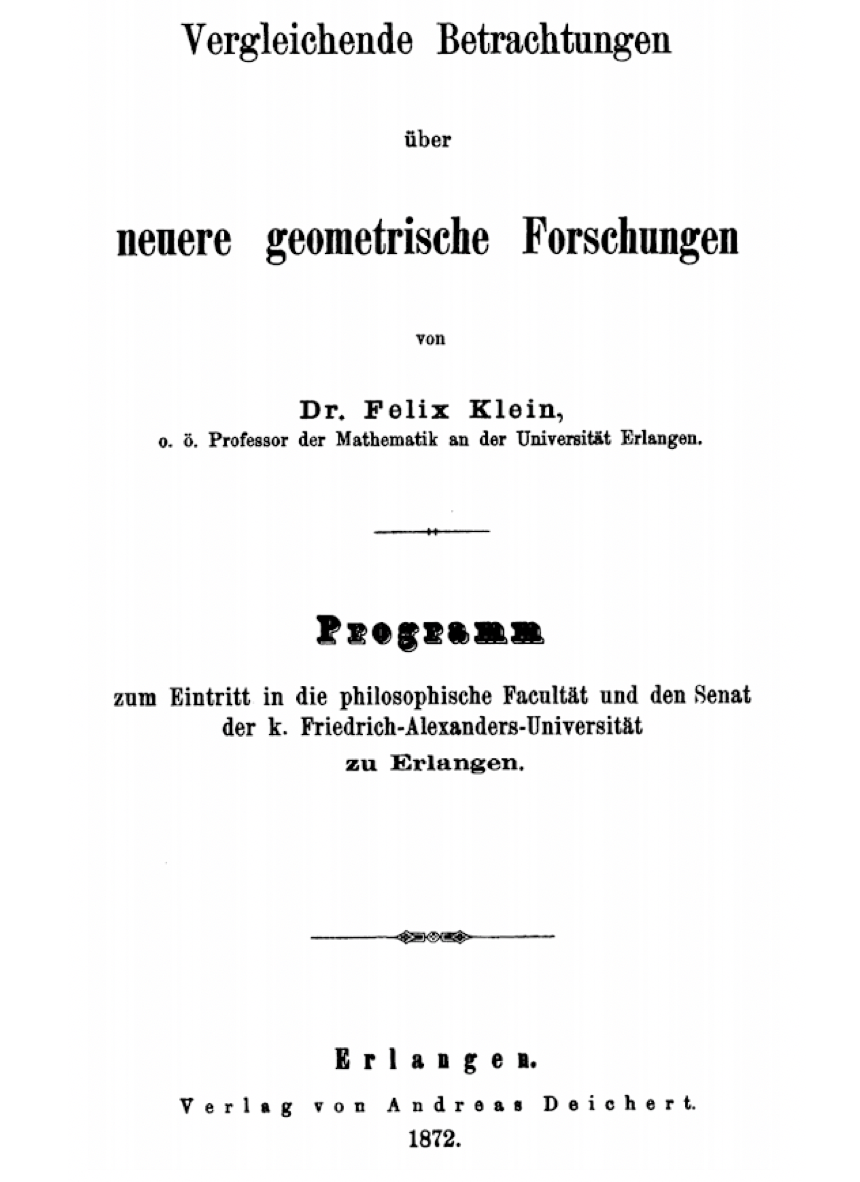
\includegraphics[width=0.9\linewidth]{figures/ml_erlangen.png}
According to a popular belief, the Erlangen Programme was delivered in Klein's inaugural address in October 1872. Klein indeed gave such a talk (though on December 7 of the same year), but it was for a non-mathematical audience and concerned primarily his ideas of mathematical education. What is now called the `Erlangen Programme' was actually a research prospectus brochure {\em Vergleichende Betrachtungen über neuere geometrische Forschungen} (``A comparative review of recent researches in geometry'') he prepared as part of his professor appointment. See \cite{tobies2019felix}. 
%, subtitled {\em Programm zum Eintritt in die philosophische Fakultät und den Senat der k. Friedrich-Alexanders-Universität zu Erlangen} (``Program for entry into the Philosophical Faculty and the Senate of the Emperor Friedrich-Alexander University of Erlangen''). 
%While Erlangen claims the credit, Klein has stayed there for only three years, moving in 1875 to the Technical University of Munich (then called {\em Technische Hochschule}), followed by Leipzig (1880), and finally settling down in Göttingen from 1886 until his retirement. See R. Tobies, Felix Klein—Mathematician, Academic Organizer, Educational Reformer, In: H. G. Weigand et al. (eds) {\em The Legacy of Felix Klein}, Springer, 2019.
} `geometry' has been synonymous with \emph{Euclidean geometry}, as no other types of geometry existed. 
%
Euclid's monopoly came to an end in the nineteenth century, with examples of non-Euclidean geometries constructed by Lobachevesky, Bolyai, Gauss, and Riemann. 
%
%By the late nineteenth century however, various alternative non-Euclidean geometries such as hyperbolic-, elliptic- and projective geometry had emerged. 
%
Towards the end of that century, these studies had diverged into disparate fields, with 
mathematicians and philosophers debating the validity of and relations between these geometries as well as the nature of the ``one true geometry''. 


A way out of this pickle was shown by a young mathematician Felix Klein, appointed in 1872 as professor in the small Bavarian University of Erlangen. In a research prospectus, which entered the annals of mathematics as the \emph{Erlangen Programme}, Klein proposed approaching geometry as the study of {\em invariants}, i.e. properties unchanged under some class of transformations, called the {\em symmetries} of the geometry.
%and used the formalism of group theory. 
%
This approach created clarity by showing that various geometries known at the time could be defined by an appropriate choice of symmetry transformations, formalized using the language of group theory. 
%
%understood as the study of those and only those properties that are invariant under some group of symmetries associated with the geometry.
For instance, Euclidean geometry is concerned with lengths and angles, because these properties are preserved by the group of Euclidean transformations (rotations and translations), while affine geometry studies parallelism, which is preserved by the group of affine transformations. 
%
The relation between these geometries is immediately apparent when considering the respective groups, because the Euclidean group is a subgroup of the affine group, which in turn is a subgroup of the group of projective transformations. 
%, so certain figures which are Euclidean-equivalent may not be affine- or projectively equivalent.


The impact of the Erlangen Programme on geometry was very profound.
Furthermore, it spilled to other fields, especially physics, where symmetry principles allowed to derive conservation laws from first principles of symmetry (an astonishing result known as Noether's Theorem), 
and even enabled the classification of elementary particles as irreducible representations of the symmetry group.
%
{\em Category theory}, 
%a formalization of abstract similarities between mathematical structures, 
now pervasive in pure mathematics,
can be ``regarded as a continuation of the Klein Erlangen Programme, in the sense that a geometrical space with its group of transformations is generalized to a category with its algebra of mappings'', in the words of its creators Samuel Eilenber and Saunders Mac Lane. \marginnote{See \cite{marquis2009category}. }


%In mathematics, the Erlangen program ultimately inspired the creation of categories by Eilenberg \& Mac Lane\footnote{Indeed, in the first paper on categories, the authors write that ``This may be regarded as a continuation of the Klein Erlanger Program, in the sense that a geometrical space with its group of transformations is generalized to a category with its algebra of mappings.''}, which are widely prized for their ability to bring forth abstract similarities between mathematical structures and to reveal many ideas as ``just'' a special case of a more general one.


At the time of writing, the state of the field of deep learning is somewhat reminiscent of the field of geometry in the nineteenth century. 
There is a veritable zoo of neural network architectures for various kinds of data, but few unifying principles. 
As in times past, this makes it difficult to understand the relations between various methods, inevitably resulting in the reinvention and re-branding of the same concepts in different application domains.  
%
For a novice trying to learn the field, absorbing the sheer volume of redundant ideas is a true nightmare.  


In this text, we make a modest attempt to apply the Erlangen Programme mindset to the domain of deep learning, with the ultimate goal of obtaining a systematisation of this field and `connecting the dots'. 
%
We call this geometrisation attempt `Geometric Deep Learning', and true to the spirit of Felix Klein, propose to derive different inductive biases and network architectures implementing them from first principles of symmetry and invariance. 
%
%more systematic understanding of the landscape of geometric deep learning methods.
%
In particular, we focus on a large class of neural networks designed for analysing unstructured sets, grids, graphs, and manifolds, and show that they can be understood in a unified manner as methods that respect the structure and symmetries of these domains. 
%
%The archetypes of these domains, grid, graphs, groups, and  `four G'


We believe this text would appeal to a broad audience of deep learning researchers, practitioners, and enthusiasts. 
%
A novice may use it as an overview and introduction to Geometric Deep Learning. 
%
A seasoned deep learning expert may discover new ways of deriving familiar architectures from basic principles and perhaps some surprising connections.  
%
Practitioners may get new insights on how to solve problems in their respective fields. 


With such a fast-paced field as modern machine learning, the risk of writing a text like this is that it becomes obsolete and irrelevant before it sees the light of day. Having focused on foundations, our hope is that the key concepts we discuss will transcend their specific realisations\marginnote{``The knowledge of certain principles easily compensates the lack of knowledge of certain facts.'' \citep{helvetius1759esprit}} --- or, as Claude Adrien Helvétius put it, {\em ``la connaissance de certains principes supplée facilement à la connoissance de certains faits.'' }

%

\section*{Notation}
\addcontentsline{toc}{section}{Notation}
\sectionmark{Notation}

\begin{minipage}{\textwidth}
\def\arraystretch{1.5}
\begin{tabular}{lp{3.25in}}
$\Omega,u$ & Domain, point on domain\\
$x(u) \in \mathcal{X}(\Omega,\mathcal{C})$ & Signal on the domain of the form $x:\Omega\rightarrow \mathcal{C}$\\
$f(x) \in \mathcal{F}(\mathcal{X}(\Omega))$ & Functions on signals on the domain of the form $f:\mathcal{X}(\Omega) \rightarrow \mathcal{Y}$\\
%
$\fG,\fg$ & Group, element of the group\\
$\fg.u, \rho(\fg)$ & Group action, group representation\\
%
$\vec{X}\in\mathcal{C}^{|\Omega|\times s}$ & Matrix representing a signal on a discrete domain\\
$\vec{x}_u\in\mathcal{C}^{s}$ & Vector representing a discrete domain signal $\vec{X}$ on element $u\in\Omega$\\
$x_{uj}\in\mathcal{C}$ & Scalar representing the $j$th component of a discrete domain signal $\vec{X}$ on element $u\in\Omega$\\
$\vec{F}(\vec{X})$ & Function on discrete domain signals that returns another discrete domain signal, as a matrix\\
%
$\tau:\Omega\rightarrow\Omega$ & Automorphism of the domain \\
$\eta:\Omega\rightarrow\Omega'$ & Isomorphism between two different domains \\
$\sigma: \mathcal{C}\rightarrow\mathcal{C}'$ & Activation function (point-wise non-linearity)\\
%
$G=(\mathcal{V},\mathcal{E})$ & Graph with nodes $\mathcal{V}$ and edges $\mathcal{E}$ \\
$\mathcal{T}=(\mathcal{V},\mathcal{E},\mathcal{F})$ & Mesh with nodes $\mathcal{V}$,  edges $\mathcal{E}$, and faces $\mathcal{F}$ \\
%
$x\star \theta$ & Convolution with filter $\theta$ \\
$S_v$ & Shift operator \\
%
$\varphi_i$ & Basis function \\
%
%
$T_u\Omega, T\Omega$ & Tangent space at $u$, tangent bundle \\
$X \in T_u\Omega$ & Tangent vector\\
$g_u(X,Y) = \langle X, Y\rangle_u$ & Riemannian metric\\
%
$\ell(\gamma), \ell_{uv}$ & Length of a curve $\gamma$, discrete metric on edge $(u,v)$ \\

\end{tabular}
\end{minipage}
\pagebreak

\section{Introduction}
Despite the well-recognized importance of training data in advancing the capabilities of large language models (LLMs)~\cite{brown2020language,kaplan2020scaling,Razeghi2022ImpactOP}, there is no agreed-upon mechanisms for crediting or compensating data providers. As LLMs are increasingly integrated into our society and economy, the absence of such mechanisms has aggravated a tension between data and model providers, exemplified by recent legal challenges involving major tech companies~\cite{jlversusalphabet,metz2022lawsuit}. In this atmosphere, data valuation, which quantifies the contribution of each training data to the model output, has been discussed as a potential technical solution for tackling these societal issues~\cite{fernandez2023data,ghorbani2019data,huang2023citation,jia2019towards,worledge2023unifying,zhao2023addressing}. 

At a high level, most data valuation algorithms interpret the model output as a coalition of its training data, and evaluate the contribution of each example based on its influence on the model output when included or excluded from the training dataset~\cite{ghorbani2019data,ilyas2022datamodels,koh2017understanding,kwon2021beta}. If an inclusion of a specific training example consistently improves model performance, high value can be assigned to this example for its contribution. However, applying existing data valuation methods to recent LLMs and their vast training datasets has faced significant scalability challenges to date. For instance, sampling-based methods, such as the Shapley value~\cite{ghorbani2019data,kwon2021beta} or Datamodels~\cite{ilyas2022datamodels}, require retraining the model multiple times with varied combinations of data subsets to directly model the effect of in/excluding each data. Unfortunately, such repeated retraining is hardly affordable even for small models, let alone LLMs. To overcome this issue, gradient-based methods, including influence functions~\cite{koh2017understanding,park2023trak}, approximate the effect of data in/exclusion on the model output using gradient information without costly retraining. Even so, scaling gradient-based methods to LLMs is hindered by prohibitive compute and memory costs originating in the high-dimensional nature of the gradient.

Consequently, the main objective of this work is to bridge the gap in scaling existing data valuation methods to recent LLMs and their vast training datasets. Toward this goal, we focus on influence functions \cite{koh2017understanding,park2023trak}, a representative gradient-based data valuation method, and significantly improve its scalability with an efficient gradient projection algorithm. We visualize the proposed data valuation system in Figure~\ref{fig:diagram}, and detail our technical contributions below:

\begin{figure}
    \centering
    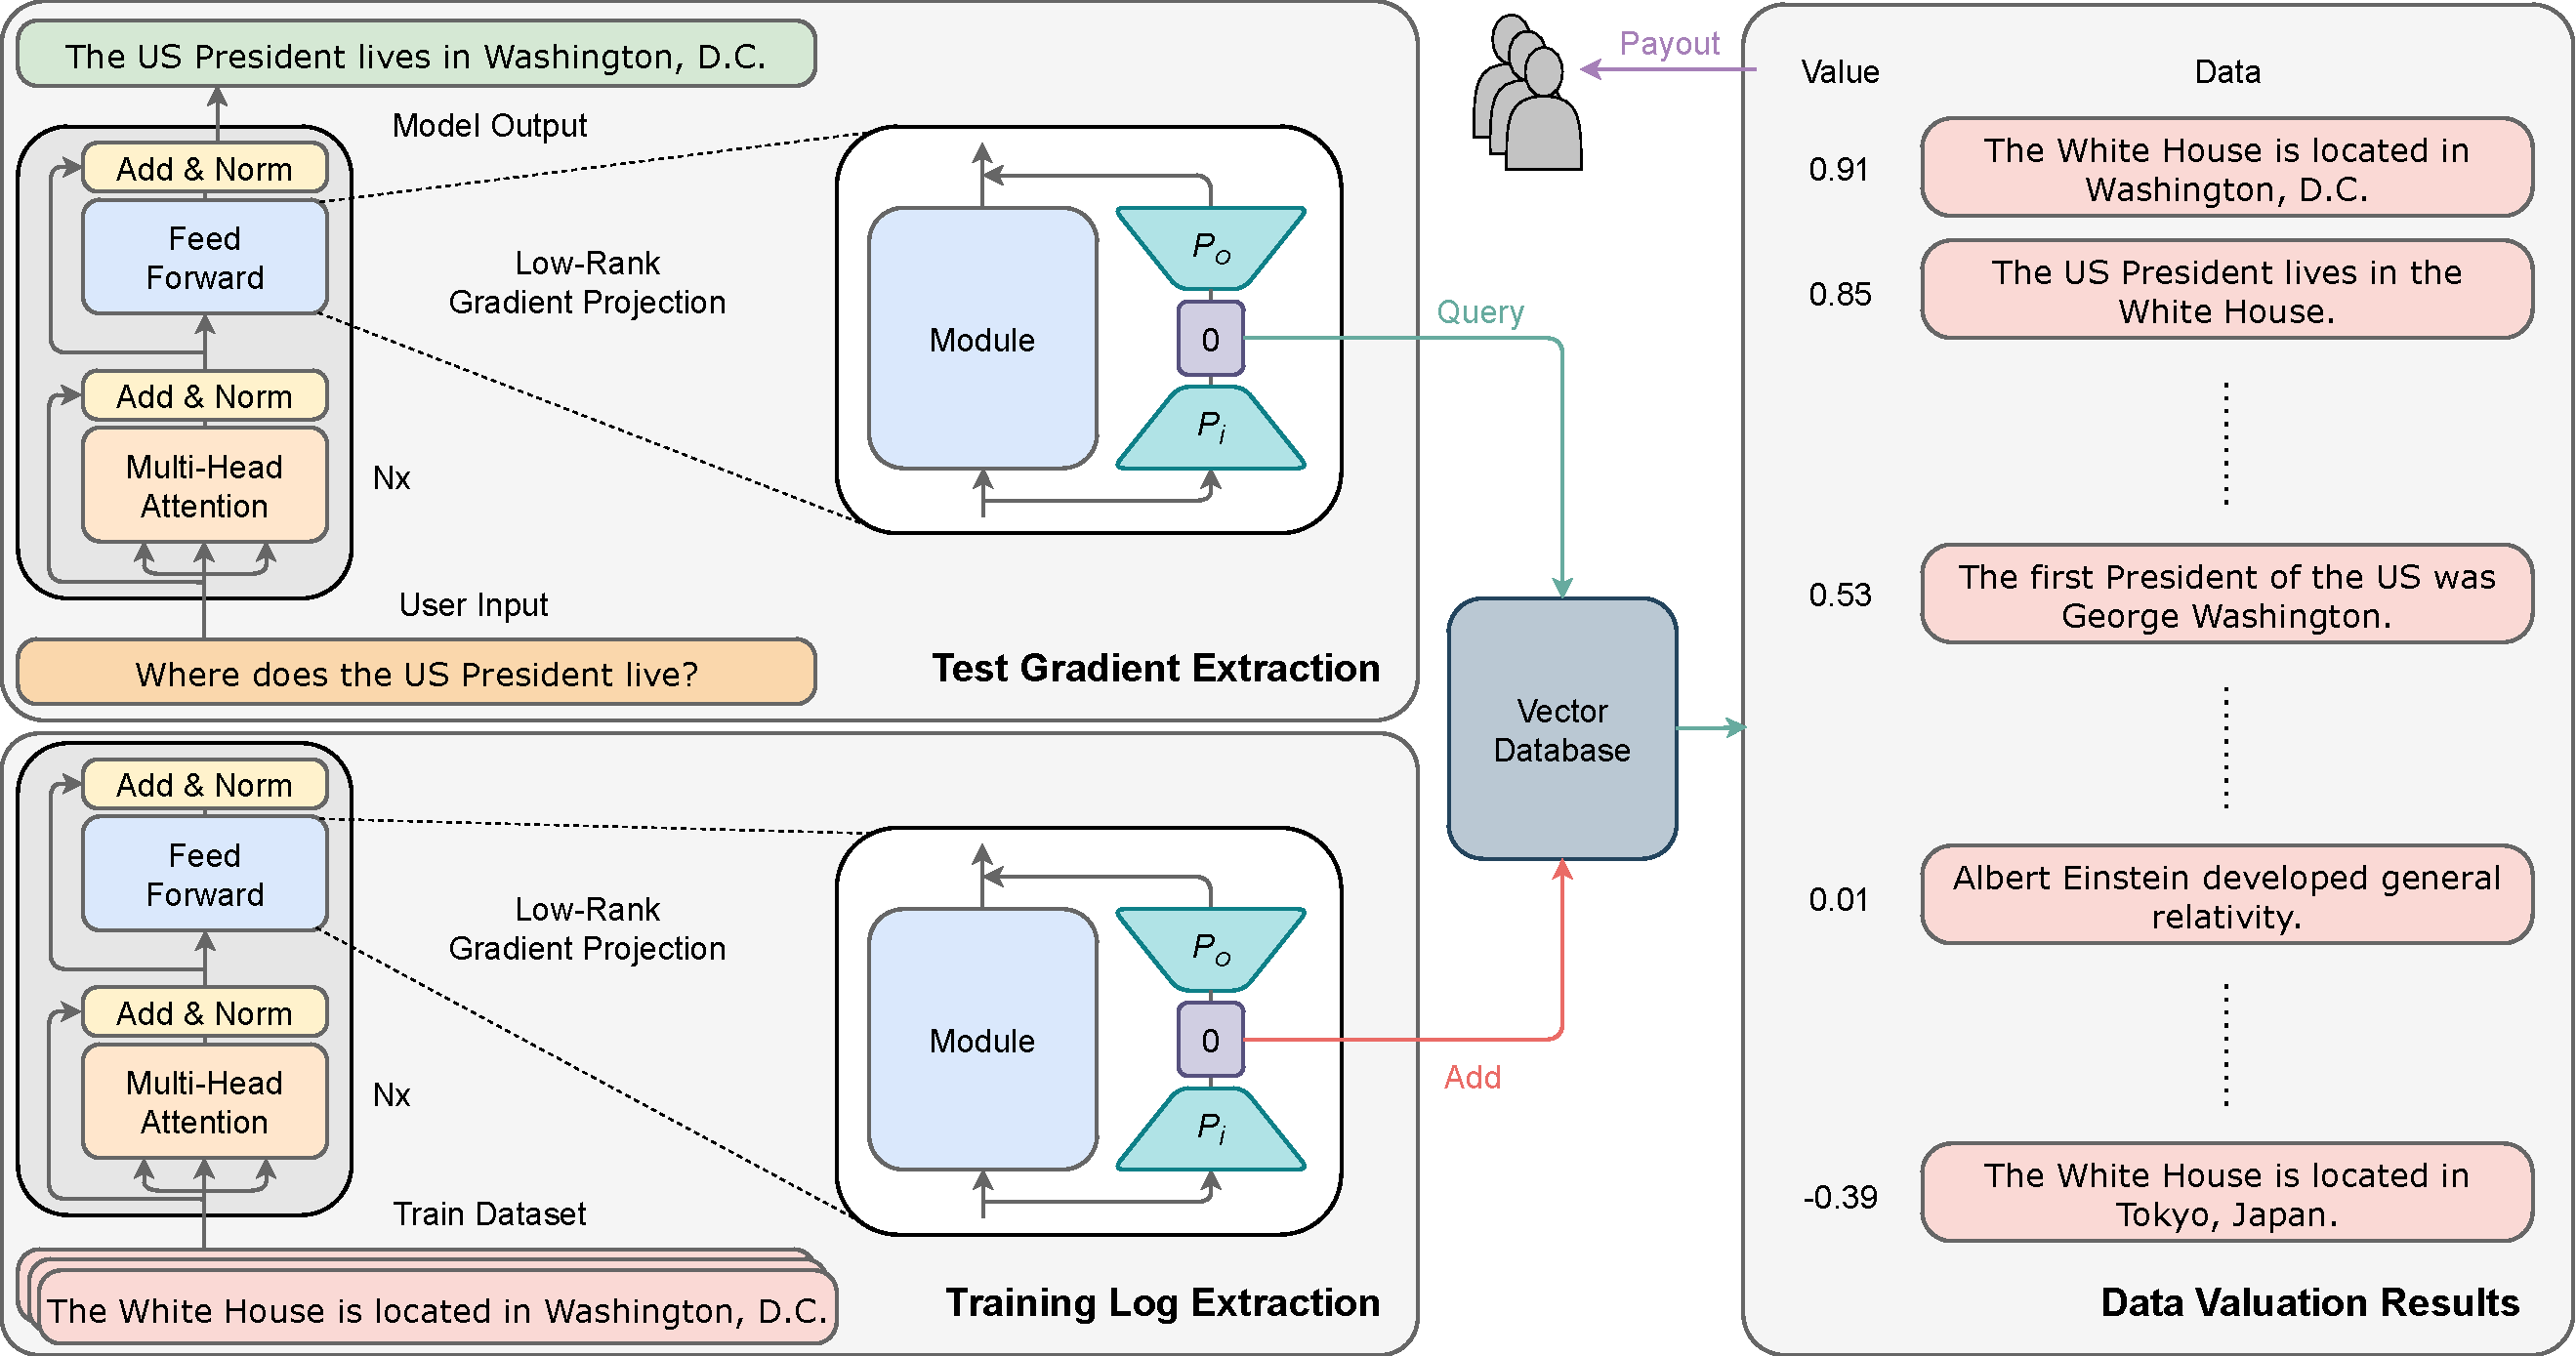
\includegraphics[width=0.94\textwidth]{figures/diagram_v7.pdf}
    \vskip -4pt
    \caption{Data valuation system architecture. \textbf{(Left Bottom)} We first extract the Hessian and gradients for all training data using efficient gradient projection \method\ and store them in a database. \textbf{(Left Top)} At test time, we similarly extract gradients and query the database. \textbf{(Right)} The database returns similarity scores with respect to training examples that can be used for data valuation/attribution.}
    \label{fig:diagram}
\end{figure}

\begin{itemize}[leftmargin=*,topsep=-2pt]
    \item Employing gradient structures in backpropagation, we develop a novel \textbf{lo}w-rank \textbf{gra}dient projection algorithm \method\ that improves space \& time complexity of gradient projection, a major scalability bottleneck in prior work~\cite{park2023trak,schioppa2022scaling}, from $O(nk)$ to $O(\sqrt{nk})$ where $n$ and $k$ are model and projection dimensions. Furthermore, \method\ directly computes projected gradients without materializing full gradients, enabling low GPU memory and high GPU utilization for improved efficiency. Lastly, we show that \method\ can be easily implemented with small add-on layers, similarly to LoRA~\cite{hu2021lora}.
    \item By interpreting a damping term in influence functions as a spectral gradient sparsification mechanism, we (1) offer a theoretical motivation of gradient projection approaches to influence functions and (2) derive a specialized PCA initialization scheme for \method.
    \item We introduce software named \software\ that (1) makes it \textit{simple} to convert existing training code into data valuation code, (2) is \textit{compatible} with various scalability tools and features in the LLM ecosystem, and (3) is \textit{extensible} to implement other data valuation or interpretability algorithms.
    \item In our data valuation experiments, \method\ demonstrates competitive accuracy against more costly baselines, while showing up to 6,500$\times$ increase in throughput and 5$\times$ reduction in GPU memory, when applied to Llama3-8B-Instruct~\cite{llama3modelcard} and the 1B-token dataset, compared to EKFAC influence \cite{grosse2023studying}, the state-of-the-art and only runnable baseline at this scale. We also observe that most valuable data identified by \method\ generally share qualitative similarities with the queried LLM output.
\end{itemize}

\bibliographystyle{plainnat}
\bibliography{references}





\end{document}                          % The required last line
